\section{Memory Access}
Having analysed the kernel symbols, we now know where data of which type is located in memory. 
Unfortunately the addresses found are virtual. The concept of virtual memory means that the physical 
locations within the built in memory chips are not accessed directly. Before accessing a virtual address 
location an address translation has to be done, which, in the case of a normal running system, 
is done automatically by the memory managing unit (MMU). 

In Linux 2.6 there are two main regions of virtual kernel space memory. One part from address 
\texttt{0x0000000000000000} to \texttt{PAGE\_OFFSET-1} (which is \texttt{0xffffffff80000000-1} 
\footnote{This numbers are valid for Kernel 2.6.27 and 2.6.28 with the default configuration 
on x86\_64 architecture.}), which can be accessed using the standard paging technique (\ref{paging}), 
the other part from \texttt{PAGE\_OFFSET} up to \texttt{0xffffffffffffffff}, is addressed using a 
linear address translation.

\subsection{Flat Kernel Memory}
\label{flat_kernel_memory}
The virtual memory area from \texttt{PAGE\_OFFSET} upwards is again divided in to two different regions. 
One from \texttt{PAGE\_OFFSET} upwards, and one from \texttt{\_\_START\_KERNEL\_map} 
\footnote{which is \texttt{0xffffffff80000000} in Linux 2.6.28 on x86\_64} upwards. 
In either case the starting address gets subtracted from the virtual address to acquire the 
physical address of the memory location inspected. All in all, we can say that regions for which 
the simple subtraction memory address translation is performed, are located in the beginning of physical memory.

\begin{lstlisting}[language=C,frame=single,caption=Accessing flat kernel memory and determine whether paging is required.,label=lst:flat_memory_access]
  if (virtual >= __START_KERNEL_map) {
  	return (virtual - __START_KERNEL_map);
  } else if(virtual >= PAGE_OFFSET) {
        return (virtual - PAGE_OFFSET);
  } else {
        // otherwise use the address lookup function
        return page_lookup(virtual);
  }
\end{lstlisting}

\subsection{Paged Kernel Memory}
\label{paging}
We have a completely different situation if we encounter paged virtual memory addresses.
Memory blocks, which are linear in virtual address space, may be distributed over several pages, which are not necessarily laid out linear in physical memory. Normally most of the kernel memory is linear accessible, because some devices that do direct memory access (DMA) require the memory region they are accessing to be linear not only in virtual, but also in physical address space. The only way to get a paged memory region in the kernel address space is to do a \texttt{vmalloc()}, which is mostly done when a bigger portion of memory is required, for example when inserting a kernel module.

When the x86\_64 machine encounters a virtual paged address, it looks up its physical page address in a page directory. 
Therefore the virtual address is divided into several parts, that index into the specific page tables (see figure \ref{page_table_structure}).

\begin{figure}[htb]
	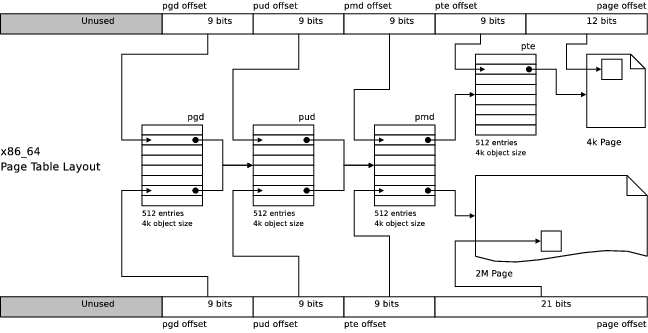
\includegraphics[width=0.95\textwidth]{imgs/x86_64_pagetable_structure.png}
	\caption{{\small Linux x86\_64 page table structure. Source: \url{http://linux-mm.org/PageTableStructure}}}
	\label{page_table_structure}
\end{figure}

As it can be seen in the figure there exist two types of pages: \texttt{4k} and \texttt{2M} pages. 
The only difference between them is their size and the indexing. For \texttt{2M} pages the last 21 bits 
of the virtual address are used to define an offset inside the page and the \texttt{pte} page directory is omitted. 
For \texttt{4k} pages the last 12 bits define a page offset and the 9 bits before that define an index 
into the 4-th level of page directory (\texttt{pte})

%Normaly this translation and lookup is done internally by a memory management unit (MMU) built into the processor. 
Since we want to access a physical memory image without having a MMU we have to emulate the accesses and 
lookups into the page directories. The entry point is the base address of the \texttt{pgd} directory. 
It is kept in the \texttt{\_\_ksymtab\_init\_level4\_pgt} kernel symbol. 
Then the virtual address is shifted successively and the lookups into the page directories are done. 

Additionally each page possesses several flags that have to be checked. One already mentioned, 
is the \texttt{PAGE\_2M} flag which identifies a \texttt{2M} page. Another important flag is the 
\texttt{PAGE\_PRESENT} flag, which is only set, if the page is allocated and available in physical memory. 
Otherwise the operating system would raise a page fault, to handle the situation accordingly. 
The third important flag would be the \texttt{PAGE\_SWAPPED} flag, which identifies that the page 
is not stored in main memory. Instead it is stored on some dedicated disk space (swap) and has to 
be loaded from there first. In our implementation swapped pages are not supported.

Every userspace program possesses its own virtual address space. Therefore separate page tables 
have to be held for each. Accessing this address is possible, if we know the process to which the address 
belongs and its pagetable location. Then a lookup can be done, just as in case of paged kernel addresses. 
In our work the focus is on analysis of kernel rootkits, therefore user space memory access is not implemented.

\section{Memory Image Comparison}
A central goal of this work is to watch memory of a virtual machine for changes and judge if malware (especially rootkits in this case) could be detected.
In order to accomplish this, two memory images (one taken before malware installation, one after) have to be compared. Usually one would compare the two physical memory dumps bytewise and try to guess if the changes happended in regions known to be security critical.
The drawback of this approach is, that one needs prior knowledge of the malware and manually create rules to detect specific malicious behaviour.
Unfortunately it is infeasible to define rules of yet unknown malware.
Therefore the opposite direction should be tried.

Instead of starting with binary differences of memory images, we start from the high level view of kernel symbols. 
For those we check whether the memory where they reside changed and if these changes reflect the behaviour of malware.

To perform a meaningful comparison two memory snapshots are opened at the same time, while our tool recursively inspects the situation: Each toplevel kernel symbol is added to a queue of symbols to compare.
The search is then conducted using a breadth first search algorithm.
Until now, the tool only reports if a specific symbol has changed.
In order to detect malware successfully, it may prove neccessary to compare the content of the changes, too.
Since the whole memory image is walked through by a python script the performance is still far from realtime. 

To implement realtime analysis for virtual machines while they are running, it could be possible that we again have to go the other way: 
Find the binary differences of the memory snapshots and abstract a high-level view of what changed without recursively checking every kernel variable.
Using our memory-coverage map, we are able to map a memory-location to a kernel variable and thus can get a list of changed variables when applying this technique to the locations found by the bin-diff tool.
While this map can be calculated in advance, this has some serious drawbacks that would need to be addressed beforehand.
If bare variables change, this is no problem, but for example in the case of pointers, 
the location of data pointed to could have changed, and therefore the value of the pointer.
This would invalidate all variables in the map to which the pointer is a parent node (in the chain from a global symbol to the variable).
One might then think of updating the mapping in iterative ways, however such algorithms remain yet to be implemented.

